\chapter[Alimentação]{Alimentação}

O fato do projeto em questão não ser autônomo implica diretamente na escolha da fonte energética do sistema. Tendo isso em mente, o abastecimento será através da rede de energia elétrica local.
Porém, visto que a rede sofre interferências externas resultando em falhas, uma proposta de aconselhável para contornar tal problema é a construção de um sistema de proteção.
Desta forma, o sistema de alimentação será então composto por um quadro de energia, este contendo todos os equipamentos necessários para a proteção dos componentes, um transformador abaixador, tendo em vista que os componentes eletrônicos trabalham com faixa máxima de tensão de 12V e um conversor CA/CC, conforme o fluxograma da figura abaixo: 

\begin{figure}[!h]
\centering
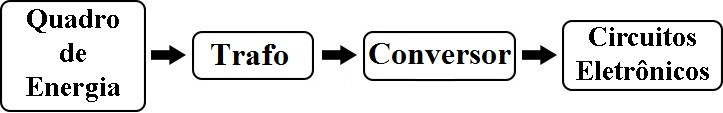
\includegraphics[scale=0.8, angle = 360]{figuras/fluxograma}
\caption[]{fluxograma esquemático da alimentação }
\end{figure}
\FloatBarrier

Os componentes a serem instalados no quadro de proteção são Botão NA, botão NF, Cabo 4mm, Conectores e Fusível.

\section{Motor}
A movimentação do robô nos eixos X e Z (considerando Y como profundidade) dependerá de motores, a qual o dimensionamento pode ser encontrado abaixo.

No eixo Z será utilizado um fuso, e a escolha do motor pode ser realizada com base na tabela abaixo:

\begin{figure}[!h]
\centering
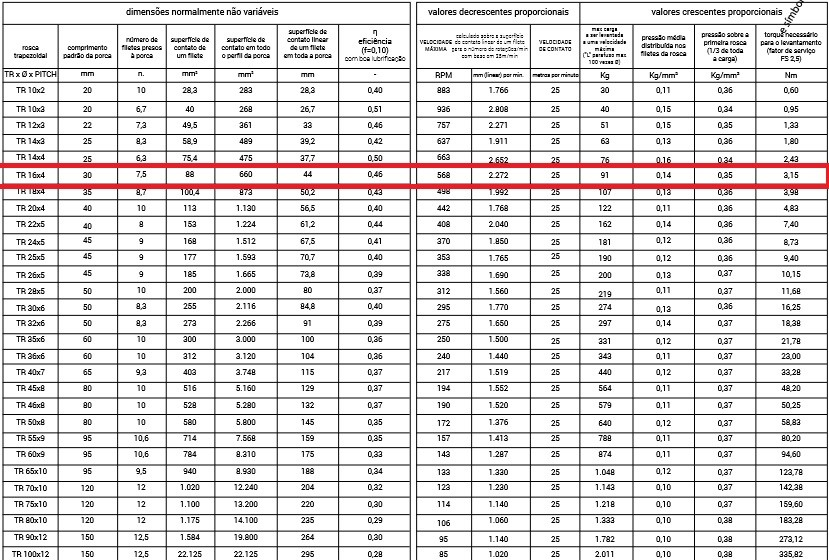
\includegraphics[scale=0.8, angle = 360]{figuras/tabela_escolha_do_motor}
\caption[]{Tabela dos dados do fuso fornecido pela estrutura}
\end{figure}
\FloatBarrier

Já no eixo X, o dimensionamento do motor é feito com base nos seguintes cálculos:

\begin{figure}[!h]
\centering
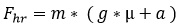
\includegraphics[scale=0.8, angle = 360]{figuras/formula1}
\caption[]{}
\end{figure}
\FloatBarrier

\begin{figure}[!h]
\centering
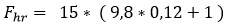
\includegraphics[scale=0.8, angle = 360]{figuras/formula2}
\caption[]{}
\end{figure}
\FloatBarrier

O coeficiente de atrito estático foi determinado como sendo\mu=0,12 , devido ao contato aço – aço. A aceleração da gravidade máxima fixada para o sistema será de 9,8m/s^2 . A massa total da estrutura da biblioteca será aproximadamente 15Kg

\begin{figure}[!h]
\centering
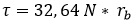
\includegraphics[scale=0.8, angle = 360]{figuras/formula3}
\caption[]{}
\end{figure}
\FloatBarrier

O raio da base de movimento equivale a 0,1m. Portanto:

\begin{figure}[!h]
\centering
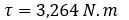
\includegraphics[scale=0.8, angle = 360]{figuras/formula4}
\caption[]{}
\end{figure}
\FloatBarrier

A velocidade estipulada pelo escopo da carga é de 0,05 m/s. Sendo assim, têm-se que a rotação do motor dimensionado será de:
 
\begin{figure}[!h]
\centering
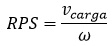
\includegraphics[scale=0.8, angle = 360]{figuras/formula5}
\caption[]{}
\end{figure}
\FloatBarrier

Por fim, RPS=0,08


\begin{figure}[!h]
\centering
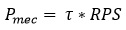
\includegraphics[scale=0.8, angle = 360]{figuras/formula7}
\caption[]{}
\end{figure}
\FloatBarrier

Finalizando, podemos obter a potência mecânica do sistema:
\begin{figure}[!h]
\centering
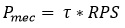
\includegraphics[scale=0.8, angle = 360]{figuras/formula8}
\caption[]{}
\end{figure}
\FloatBarrier


A escolha de um motor com torque aproximado à 
32,64Kgf.cm por valores superiores é aconselhável, desta forma, o motor NEMA 23 com caixa de redução foi escolhido.

\begin{figure}[!h]
\centering
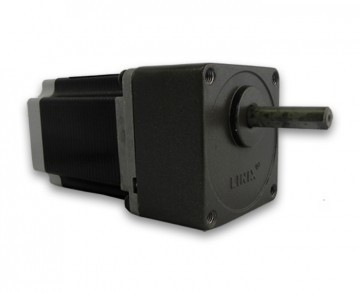
\includegraphics[scale=0.8, angle = 360]{figuras/Motor}
\caption[]{}
\end{figure}
\FloatBarrier

\begin{figure}[!h]
\centering
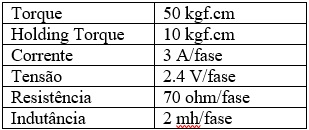
\includegraphics[scale=0.8, angle = 360]{figuras/tabela_unipolar}
\caption[]{}
\end{figure}
\FloatBarrier

